\chapter{Controller System}\label{sec:controller_sys}
\href{http://ctms.engin.umich.edu/CTMS/index.php?example=MotorPosition&section=SystemModeling}{DC Motor Position: System Modeling}


??????????????? We need this ????????????????

ORLANDO will use it later maybe.

\subsection{Physical Setup}
A common actuator in control systems is the DC motor. It directly provides rotary motion and, coupled with wheels or drums and cables, can provide translational motion. The electric equivalent circuit of the armature and the free-body diagram of the rotor are shown in the following figure. 

\begin{figure}[h!]\label{fig:motor_model}
	\centering
	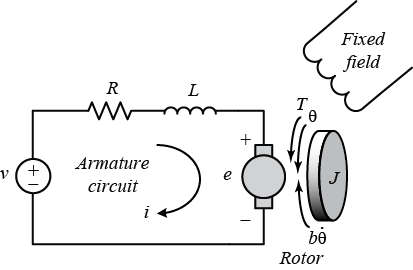
\includegraphics[width=0.7\textwidth]{figures/motor.png}
	\caption{DC Servo Motor}
\end{figure}

From the figure above, we can derive the following governing equations based on Newton's 2nd law and Kirchhoff's voltage law.

\begin{equation}
	J \dot{\dot{\Theta}} + b\dot{\Theta} = Ki \\
	L\frac{di}{dt} + Ri = V - K\dot{\Theta}
\end{equation}

\subsection{Transfer Function}
Applying the Laplace transform, the above modeling equations can be expressed in terms of the Laplace variable s. On the link they do not consider initial condition and we want them.

\begin{equation}
	\mathscr{L}\{J \dot{\dot{\Theta}}\}  + \mathscr{L}\{b\dot{\Theta}\} = \mathscr{L}\{Ki\}
\end{equation}

The result become:
\begin{align*}
	& L(I(s)s-i(0)) + RI(s) = V(s) - K(s\Theta (s) - \theta (0)) \\
	& \Rightarrow I(s)(Ls+R) = V(s) - K(s\Theta (s) - \theta (0)) +Li(0) \\
	& \Rightarrow I(s) = \frac{V(s) - K(s\Theta (s) - \theta (0)) +Li(0)}{(Ls+R)}
\end{align*}

Kirchoffs voltage law:
\begin{equation*}
	\mathscr{L}\{L\frac{di}{dt}\} + \mathscr{L}\{Ri\} = \mathscr{L}\{V\} - \mathscr{L}\{K\dot{\Theta}\}
\end{equation*}

The result become:
\begin{align*}
	& J(s^2 \Theta(s) - s\theta (0) - \dot{\theta} (0)) +b(s\Theta (s)-\theta (0)) = KI(s) \\
	& Js^2 J\Theta(s) - Js\theta (0) - J\dot{\theta} (0) +b(s\Theta (s)-\theta (0) = KI(s) 
\end{align*}

And with I(s) inserted:
\begin{align*}
	& Js^2 J\Theta(s) - Js\theta (0) - J\dot{\theta} (0) +b(s\Theta (s)-\theta (0) = K (\frac{V(s) - K(s\Theta (s) - \theta (0)) +Li(0)}{(Ls+R)}) \\
	& (Js^2 J\Theta(s) - Js\theta (0) - J\dot{\theta} (0) +b(s\Theta (s)-\theta (0))(Ls+R) =  K(V(s) - K(s\Theta (s) - \theta (0)) +Li(0)) \\
	& \Theta(s)(Js^2 J +bs) - Js\theta (0) - J\dot{\theta} (0) -\theta (0))(Ls+R) =  K(V(s) - K(s\Theta (s) - \theta (0)) +Li(0))
\end{align*}

And then...
\begin{align*}
	& \Theta(s)((Ls+R)(Js^2 J +bs)+K^2s) + \\
	& (Ls+R)(-Js\theta (0) - J\dot{\theta} (0) -b\theta (0)) = KV(s) - K^2 \theta (0) +KLi(0)
\end{align*}

And then...
\begin{align*}
	\Theta(s) &= \frac{KV(s) - K^2 \theta (0) +KLi(0) - (Ls+R)(-Js\theta (0) - J\dot{\theta} (0) -b\theta (0))}{(Ls+R)(Js^2 J +bs)+K^2s} \\
			  &= \frac{K}{(Ls+R)(Js^2 J +bs)+K^2s}V(s) + \\
	          &\frac{KV(s) - K^2 \theta (0) +KLi(0) - (Ls+R)(-Js\theta (0) - J\dot{\theta} (0) -b\theta (0))}{(Ls+R)(Js^2 J +bs)+K^2s}
\end{align*}